\experiment{Disk Schedule Algorithms}{11/10/2023}

\section{Aim}
Simulate disk scheduling algorithms: a)FCFS b)SCAN c)C-SCAN

\section{Algorithm}
\subsection{FCFS}
\begin{enumerate}
    \item Start
    \item Input the number of requests to $n$.
    \item Input requests to array $req$.
    \item Input head position to variable $head$.
    \item Iterate through the $req$ array and do the following:
    \begin{enumerate}
        \item Print the current request value $req[i]$.
        \item Calculate the absolute difference between the current request and the head position and add it to $d$.
        \item Update the head position with the current request value.
    \end{enumerate}
    \item Display seek count $d$.
    \item Stop
\end{enumerate}

\subsection{SCAN}
\begin{enumerate}
    \item Start
    \item Input the number of requests to $n$.
    \item Input requests to array $req$.
    \item Input max track no and head position to variable $max$ and $head$.
    \item Sort the $req[]$ array in ascending order.
    \item Set $l$ to $n-1$.
    \item Iterate through the $req$ array and if the current request value is greater than or equal to the head position, set $l$ to $i$ and break the loop.
    \item Set $d = max - head + max - req[0]$.
    \item Use a loop to print the request values from $l$ to $n-1$, representing the forward seek sequence.
    \begin{enumerate}
        \item Print the current request value $req[i]$.
        \item Update the head position with the current request value.
    \end{enumerate}
    \item Use a loop to print the request values from $l-1$ to $1$, representing the backward seek sequence.
    \begin{enumerate}
        \item Print the current request value $req[i]$.
        \item Update the head position with the current request value.
    \end{enumerate}
    \item Print the first request value $req[0]$.
    \item Display seek count $d$.
    \item Stop
\end{enumerate}

\subsection{C-SCAN}
\begin{enumerate}
    \item Start
    \item Input the number of requests to $n$.
    \item Input requests to array $req$.
    \item Input max track no and head position to variable $max$ and $head$.
    \item Sort the $req[]$ array in ascending order.
    \item Set $l$ to $n-1$.
    \item Iterate through the $req$ array and if the current request value is greater than or equal to the head position, set $l$ to $i$ and break the loop.
    \item Set $d = max - head + max + req[l-1]$.
    \item Use a loop to print the request values from $l$ to $n-1$, representing the forward seek sequence.
    \begin{enumerate}
        \item Print the current request value $req[i]$.
        \item Update the head position with the current request value.
    \end{enumerate}
    \item Print "0-->
" to represent the seek to track 0.
    \item Use a loop to print the request values from 0 to $l-1$, representing the backward seek sequence.
    \begin{enumerate}
        \item Print the current request value $req[l-1]$.
        \item Update the head position with the current request value.
    \end{enumerate}
    \item Print the first request value $req[0]$.
    \item Display seek count $d$.
    \item Stop
\end{enumerate}


\section{C Program}

\subsection{FCFS}
\begin{lstlisting}[label={list:c_program:queue}]
#include <stdio.h>
#include <stdlib.h>
#include <math.h>

int main()
{
    int n, req[10], head, count = 0, d = 0;

    printf("Enter the number of requests: ");
    scanf("%d", &n);

    printf("Enter the requests: ");
    for (int i = 0; i < n; i++)
    {
        scanf("%d", &req[i]);
    }

    printf("Enter the head position: ");
    scanf("%d", &head);

    printf("Seek Sequence: ");
    for (int i = 0; i < n - 1; i++)
    {
        printf("%d --> ", req[i]);
        d += abs(req[i] - head);
        head = req[i];
    }

    printf("%d", req[n - 1]);
    d += abs(req[n - 1] - head);

    printf("\nSeek Count is: %d\n", d);

    return 0;
}

\end{lstlisting}
\subsection{SCAN}
\begin{lstlisting}[label={list:c_program:queue}]
#include <stdio.h>
#include <stdlib.h>

int main()
{
    int n, max, req[10], head, count = 0, d = 0, t, l;

    printf("Enter the number of requests: ");
    scanf("%d", &n);

    printf("Enter the requests: ");
    for (int i = 0; i < n; i++)
    {
        scanf("%d", &req[i]);
    }

    printf("Enter the max track number: ");
    scanf("%d", &max);

    printf("Enter the head position: ");
    scanf("%d", &head);

    for (int i = 0; i < n; i++)
    {
        for (int j = 0; j < n - i - 1; j++)
        {
            if (req[j] > req[j + 1])
            {
                t = req[j];
                req[j] = req[j + 1];
                req[j + 1] = t;
            }
        }
    }

    l = n - 1;
    for (int i = 0; i < n; i++)
    {
        if (req[i] >= head)
        {
            l = i;
            break;
        }
    }

    d = max - head + max + req[l - 1];

    printf("Seek Sequence: ");

    for (int i = l; i < n; i++)
    {
        printf("%d --> ", req[i]);
        head = req[i];
    }

    printf("0 --> "); // Seek to track 0

    for (int i = 0; i < l; i++)
    {
        printf("%d --> ", req[i]);
        head = req[i];
    }

    printf("%d", req[l]);

    printf("\nSeek Count is: %d\n", d);

    return 0;
}
\end{lstlisting}

\subsection{CSCAN}
\begin{lstlisting}[label={list:c_program:queue}]
#include <stdio.h>
#include <stdlib.h>

void main() {
    int n, max, req[10], head, count = 0, d = 0, t, l;

    printf("Enter no of requests:");
    scanf("%d", &n);
    printf("Enter the requests:");
    for (int i = 0; i < n; i++) {
        scanf("%d", &req[i]);
    }
    printf("Enter max track no:");
    scanf("%d", &max);
    printf("Enter head position:");
    scanf("%d", &head);

    for (int i = 0; i < n; i++) {
        for (int j = 0; j < n - i - 1; j++) {
            if (req[j] > req[j + 1]) {
                t = req[j];
                req[j] = req[j + 1];
                req[j + 1] = t;
            }
        }
    }

    l = n - 1;
    for (int i = 0; i < n; i++) {
        if (req[i] >= head) {
            l = i;
            break;
        }
    }

    d = max - head + max + req[l - 1];
    printf("Seek Sequence :");
    for (int i = l; i < n; i++) {
        printf("%d-->", req[i]);
        head = req[i];
    }
    printf("0-->");
    for (int i = 0; i < l - 1; i++) {
        printf("%d-->", req[i]);
        head = req[i];
    }
    printf("%d", req[l - 1]);
    printf("\nSeek Count is:%d\n", d);
}
\end{lstlisting}


\section{Output}
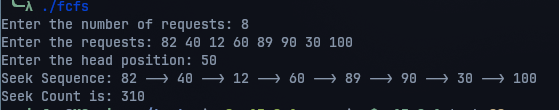
\includegraphics[]{Cycle_4//Outputs/fcfs1.png}
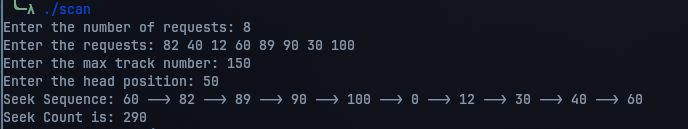
\includegraphics[]{Cycle_4//Outputs/scan.png}
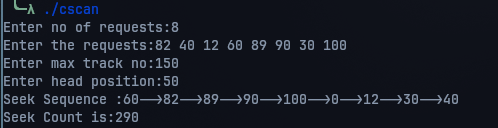
\includegraphics[]{Cycle_4//Outputs/cscan.png}


\section{Result}
Executed Disk Scheduling Algorithms successfully